\documentclass[1p]{elsarticle_modified}
%\bibliographystyle{elsarticle-num}

%\usepackage[colorlinks]{hyperref}
%\usepackage{abbrmath_seonhwa} %\Abb, \Ascr, \Acal ,\Abf, \Afrak
\usepackage{amsfonts}
\usepackage{amssymb}
\usepackage{amsmath}
\usepackage{amsthm}
\usepackage{scalefnt}
\usepackage{amsbsy}
\usepackage{kotex}
\usepackage{caption}
\usepackage{subfig}
\usepackage{color}
\usepackage{graphicx}
\usepackage{xcolor} %% white, black, red, green, blue, cyan, magenta, yellow
\usepackage{float}
\usepackage{setspace}
\usepackage{hyperref}

\usepackage{tikz}
\usetikzlibrary{arrows}

\usepackage{multirow}
\usepackage{array} % fixed length table
\usepackage{hhline}

%%%%%%%%%%%%%%%%%%%%%
\makeatletter
\renewcommand*\env@matrix[1][\arraystretch]{%
	\edef\arraystretch{#1}%
	\hskip -\arraycolsep
	\let\@ifnextchar\new@ifnextchar
	\array{*\c@MaxMatrixCols c}}
\makeatother %https://tex.stackexchange.com/questions/14071/how-can-i-increase-the-line-spacing-in-a-matrix
%%%%%%%%%%%%%%%

\usepackage[normalem]{ulem}

\newcommand{\msout}[1]{\ifmmode\text{\sout{\ensuremath{#1}}}\else\sout{#1}\fi}
%SOURCE: \msout is \stkout macro in https://tex.stackexchange.com/questions/20609/strikeout-in-math-mode

\newcommand{\cancel}[1]{
	\ifmmode
	{\color{red}\msout{#1}}
	\else
	{\color{red}\sout{#1}}
	\fi
}

\newcommand{\add}[1]{
	{\color{blue}\uwave{#1}}
}

\newcommand{\replace}[2]{
	\ifmmode
	{\color{red}\msout{#1}}{\color{blue}\uwave{#2}}
	\else
	{\color{red}\sout{#1}}{\color{blue}\uwave{#2}}
	\fi
}

\newcommand{\Sol}{\mathcal{S}} %segment
\newcommand{\D}{D} %diagram
\newcommand{\A}{\mathcal{A}} %arc


%%%%%%%%%%%%%%%%%%%%%%%%%%%%%5 test

\def\sl{\operatorname{\textup{SL}}(2,\Cbb)}
\def\psl{\operatorname{\textup{PSL}}(2,\Cbb)}
\def\quan{\mkern 1mu \triangleright \mkern 1mu}

\theoremstyle{definition}
\newtheorem{thm}{Theorem}[section]
\newtheorem{prop}[thm]{Proposition}
\newtheorem{lem}[thm]{Lemma}
\newtheorem{ques}[thm]{Question}
\newtheorem{cor}[thm]{Corollary}
\newtheorem{defn}[thm]{Definition}
\newtheorem{exam}[thm]{Example}
\newtheorem{rmk}[thm]{Remark}
\newtheorem{alg}[thm]{Algorithm}

\newcommand{\I}{\sqrt{-1}}
\begin{document}

%\begin{frontmatter}
%
%\title{Boundary parabolic representations of knots up to 8 crossings}
%
%%% Group authors per affiliation:
%\author{Yunhi Cho} 
%\address{Department of Mathematics, University of Seoul, Seoul, Korea}
%\ead{yhcho@uos.ac.kr}
%
%
%\author{Seonhwa Kim} %\fnref{s_kim}}
%\address{Center for Geometry and Physics, Institute for Basic Science, Pohang, 37673, Korea}
%\ead{ryeona17@ibs.re.kr}
%
%\author{Hyuk Kim}
%\address{Department of Mathematical Sciences, Seoul National University, Seoul 08826, Korea}
%\ead{hyukkim@snu.ac.kr}
%
%\author{Seokbeom Yoon}
%\address{Department of Mathematical Sciences, Seoul National University, Seoul, 08826,  Korea}
%\ead{sbyoon15@snu.ac.kr}
%
%\begin{abstract}
%We find all boundary parabolic representation of knots up to 8 crossings.
%
%\end{abstract}
%\begin{keyword}
%    \MSC[2010] 57M25 
%\end{keyword}
%
%\end{frontmatter}

%\linenumbers
%\tableofcontents
%
\newcommand\colored[1]{\textcolor{white}{\rule[-0.35ex]{0.8em}{1.4ex}}\kern-0.8em\color{red} #1}%
%\newcommand\colored[1]{\textcolor{white}{ #1}\kern-2.17ex	\textcolor{white}{ #1}\kern-1.81ex	\textcolor{white}{ #1}\kern-2.15ex\color{red}#1	}

{\Large $\underline{11a_{337}~(K11a_{337})}$}

\setlength{\tabcolsep}{10pt}
\renewcommand{\arraystretch}{1.6}
\vspace{1cm}\begin{tabular}{m{100pt}>{\centering\arraybackslash}m{274pt}}
\multirow{5}{120pt}{
	\centering
	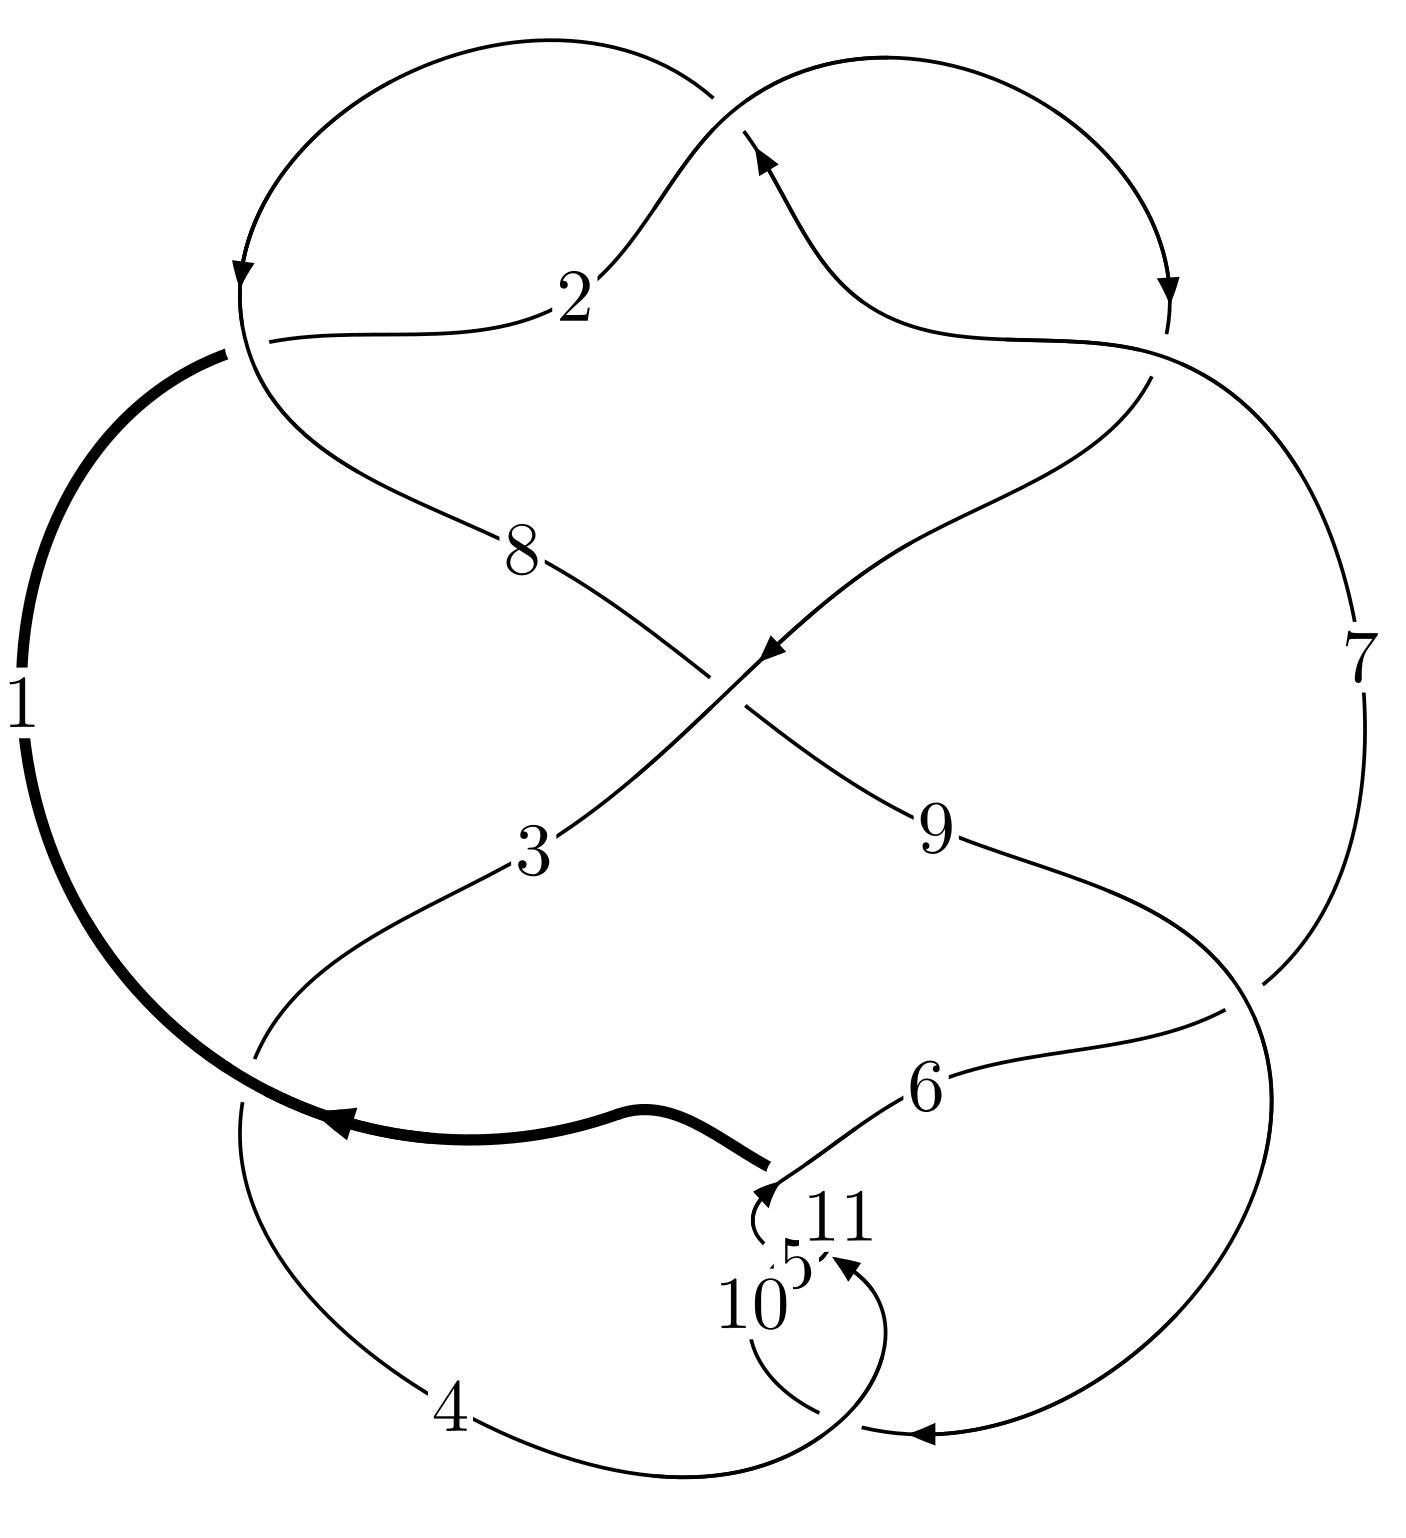
\includegraphics[width=112pt]{../../../GIT/diagram.site/Diagrams/png/586_11a_337.png}\\
\ \ \ A knot diagram\footnotemark}&
\allowdisplaybreaks
\textbf{Linearized knot diagam} \\
\cline{2-2}
 &
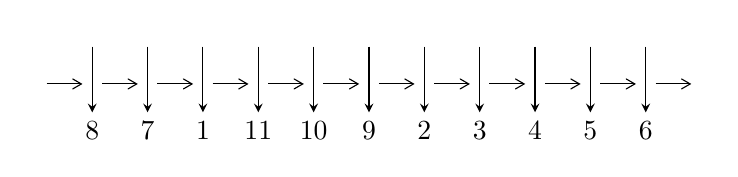
\begin{tikzpicture}[x=20pt, y=17pt]
	% nodes
	\node (C0) at (0, 0) {};
	\node (C1) at (1, 0) {};
	\node (C1U) at (1, +1) {};
	\node (C1D) at (1, -1) {8};

	\node (C2) at (2, 0) {};
	\node (C2U) at (2, +1) {};
	\node (C2D) at (2, -1) {7};

	\node (C3) at (3, 0) {};
	\node (C3U) at (3, +1) {};
	\node (C3D) at (3, -1) {1};

	\node (C4) at (4, 0) {};
	\node (C4U) at (4, +1) {};
	\node (C4D) at (4, -1) {11};

	\node (C5) at (5, 0) {};
	\node (C5U) at (5, +1) {};
	\node (C5D) at (5, -1) {10};

	\node (C6) at (6, 0) {};
	\node (C6U) at (6, +1) {};
	\node (C6D) at (6, -1) {9};

	\node (C7) at (7, 0) {};
	\node (C7U) at (7, +1) {};
	\node (C7D) at (7, -1) {2};

	\node (C8) at (8, 0) {};
	\node (C8U) at (8, +1) {};
	\node (C8D) at (8, -1) {3};

	\node (C9) at (9, 0) {};
	\node (C9U) at (9, +1) {};
	\node (C9D) at (9, -1) {4};

	\node (C10) at (10, 0) {};
	\node (C10U) at (10, +1) {};
	\node (C10D) at (10, -1) {5};

	\node (C11) at (11, 0) {};
	\node (C11U) at (11, +1) {};
	\node (C11D) at (11, -1) {6};
	\node (C12) at (12, 0) {};

	% arrows
	\draw[->,>={angle 60}]
	(C0) edge (C1) (C1) edge (C2) (C2) edge (C3) (C3) edge (C4) (C4) edge (C5) (C5) edge (C6) (C6) edge (C7) (C7) edge (C8) (C8) edge (C9) (C9) edge (C10) (C10) edge (C11) (C11) edge (C12) ;	\draw[->,>=stealth]
	(C1U) edge (C1D) (C2U) edge (C2D) (C3U) edge (C3D) (C4U) edge (C4D) (C5U) edge (C5D) (C6U) edge (C6D) (C7U) edge (C7D) (C8U) edge (C8D) (C9U) edge (C9D) (C10U) edge (C10D) (C11U) edge (C11D) ;
	\end{tikzpicture} \\
\hhline{~~} \\& 
\textbf{Solving Sequence} \\ \cline{2-2} 
 &
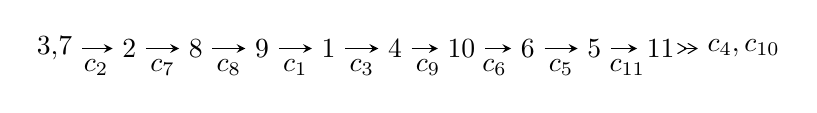
\begin{tikzpicture}[x=24pt, y=7pt]
	% node
	\node (A0) at (-1/8, 0) {3,7};
	\node (A1) at (1, 0) {2};
	\node (A2) at (2, 0) {8};
	\node (A3) at (3, 0) {9};
	\node (A4) at (4, 0) {1};
	\node (A5) at (5, 0) {4};
	\node (A6) at (6, 0) {10};
	\node (A7) at (7, 0) {6};
	\node (A8) at (8, 0) {5};
	\node (A9) at (9, 0) {11};
	\node (C1) at (1/2, -1) {$c_{2}$};
	\node (C2) at (3/2, -1) {$c_{7}$};
	\node (C3) at (5/2, -1) {$c_{8}$};
	\node (C4) at (7/2, -1) {$c_{1}$};
	\node (C5) at (9/2, -1) {$c_{3}$};
	\node (C6) at (11/2, -1) {$c_{9}$};
	\node (C7) at (13/2, -1) {$c_{6}$};
	\node (C8) at (15/2, -1) {$c_{5}$};
	\node (C9) at (17/2, -1) {$c_{11}$};
	\node (A10) at (41/4, 0) {$c_{4},c_{10}$};

	% edge
	\draw[->,>=stealth]	
	(A0) edge (A1) (A1) edge (A2) (A2) edge (A3) (A3) edge (A4) (A4) edge (A5) (A5) edge (A6) (A6) edge (A7) (A7) edge (A8) (A8) edge (A9) ;
	\draw[->>,>={angle 60}]	
	(A9) edge (A10);
\end{tikzpicture} \\ 

\end{tabular} \\

\footnotetext{
The image of knot diagram is generated by the software ``\textbf{Draw programme}" developed by Andrew Bartholomew(\url{http://www.layer8.co.uk/maths/draw/index.htm\#Running-draw}), where we modified some parts for our purpose(\url{https://github.com/CATsTAILs/LinksPainter}).
}\phantom \\ \newline 
\centering \textbf{Ideals for irreducible components\footnotemark of $X_{\text{par}}$} 
 
\begin{align*}
I^u_{1}&=\langle 
u^{44}+u^{43}+\cdots+5 u^2-1\rangle \\
\\
\end{align*}
\raggedright * 1 irreducible components of $\dim_{\mathbb{C}}=0$, with total 44 representations.\\
\footnotetext{All coefficients of polynomials are rational numbers. But the coefficients are sometimes approximated in decimal forms when there is not enough margin.}
\newpage
\renewcommand{\arraystretch}{1}
\centering \section*{I. $I^u_{1}= \langle u^{44}+u^{43}+\cdots+5 u^2-1 \rangle$}
\flushleft \textbf{(i) Arc colorings}\\
\begin{tabular}{m{7pt} m{180pt} m{7pt} m{180pt} }
\flushright $a_{3}=$&$\begin{pmatrix}1\\0\end{pmatrix}$ \\
\flushright $a_{7}=$&$\begin{pmatrix}0\\u\end{pmatrix}$ \\
\flushright $a_{2}=$&$\begin{pmatrix}1\\- u^2\end{pmatrix}$ \\
\flushright $a_{8}=$&$\begin{pmatrix}- u\\u^3+u\end{pmatrix}$ \\
\flushright $a_{9}=$&$\begin{pmatrix}- u^3-2 u\\u^3+u\end{pmatrix}$ \\
\flushright $a_{1}=$&$\begin{pmatrix}u^2+1\\- u^4-2 u^2\end{pmatrix}$ \\
\flushright $a_{4}=$&$\begin{pmatrix}- u^6-3 u^4-2 u^2+1\\u^8+4 u^6+4 u^4\end{pmatrix}$ \\
\flushright $a_{10}=$&$\begin{pmatrix}u^{17}+8 u^{15}+25 u^{13}+36 u^{11}+19 u^9-4 u^7-2 u^5+2 u^3-3 u\\- u^{19}-9 u^{17}-32 u^{15}-55 u^{13}-43 u^{11}-9 u^9-4 u^5+u^3+u\end{pmatrix}$ \\
\flushright $a_{6}=$&$\begin{pmatrix}u^7+4 u^5+4 u^3\\- u^7-3 u^5-2 u^3+u\end{pmatrix}$ \\
\flushright $a_{5}=$&$\begin{pmatrix}u^{43}+20 u^{41}+\cdots-14 u^5+13 u^3\\- u^{43}- u^{42}+\cdots-5 u^2+1\end{pmatrix}$ \\
\flushright $a_{11}=$&$\begin{pmatrix}- u^{18}-9 u^{16}-32 u^{14}-55 u^{12}-43 u^{10}-9 u^8-4 u^4+u^2+1\\u^{18}+8 u^{16}+25 u^{14}+36 u^{12}+19 u^{10}-4 u^8-2 u^6+2 u^4-3 u^2\end{pmatrix}$\\ \flushright $a_{11}=$&$\begin{pmatrix}- u^{18}-9 u^{16}-32 u^{14}-55 u^{12}-43 u^{10}-9 u^8-4 u^4+u^2+1\\u^{18}+8 u^{16}+25 u^{14}+36 u^{12}+19 u^{10}-4 u^8-2 u^6+2 u^4-3 u^2\end{pmatrix}$\\&\end{tabular}
\flushleft \textbf{(ii) Obstruction class $= -1$}\\~\\
\flushleft \textbf{(iii) Cusp Shapes $= -4 u^{42}-4 u^{41}+\cdots-20 u-10$}\\~\\
\newpage\renewcommand{\arraystretch}{1}
\flushleft \textbf{(iv) u-Polynomials at the component}\newline \\
\begin{tabular}{m{50pt}|m{274pt}}
Crossings & \hspace{64pt}u-Polynomials at each crossing \\
\hline $$\begin{aligned}c_{1},c_{2},c_{7}\end{aligned}$$&$\begin{aligned}
&u^{44}- u^{43}+\cdots+5 u^2-1
\end{aligned}$\\
\hline $$\begin{aligned}c_{3},c_{6}\end{aligned}$$&$\begin{aligned}
&u^{44}-7 u^{43}+\cdots-96 u+17
\end{aligned}$\\
\hline $$\begin{aligned}c_{4},c_{5},c_{10}\end{aligned}$$&$\begin{aligned}
&u^{44}+u^{43}+\cdots-2 u-1
\end{aligned}$\\
\hline $$\begin{aligned}c_{8}\end{aligned}$$&$\begin{aligned}
&u^{44}+u^{43}+\cdots+20 u-53
\end{aligned}$\\
\hline $$\begin{aligned}c_{9},c_{11}\end{aligned}$$&$\begin{aligned}
&u^{44}- u^{43}+\cdots+5 u^2-1
\end{aligned}$\\
\hline
\end{tabular}\\~\\
\newpage\renewcommand{\arraystretch}{1}
\flushleft \textbf{(v) Riley Polynomials at the component}\newline \\
\begin{tabular}{m{50pt}|m{274pt}}
Crossings & \hspace{64pt}Riley Polynomials at each crossing \\
\hline $$\begin{aligned}c_{1},c_{2},c_{7}\end{aligned}$$&$\begin{aligned}
&y^{44}+41 y^{43}+\cdots-10 y+1
\end{aligned}$\\
\hline $$\begin{aligned}c_{3},c_{6}\end{aligned}$$&$\begin{aligned}
&y^{44}+33 y^{43}+\cdots-1770 y+289
\end{aligned}$\\
\hline $$\begin{aligned}c_{4},c_{5},c_{10}\end{aligned}$$&$\begin{aligned}
&y^{44}+37 y^{43}+\cdots-10 y+1
\end{aligned}$\\
\hline $$\begin{aligned}c_{8}\end{aligned}$$&$\begin{aligned}
&y^{44}+13 y^{43}+\cdots+8822 y+2809
\end{aligned}$\\
\hline $$\begin{aligned}c_{9},c_{11}\end{aligned}$$&$\begin{aligned}
&y^{44}-23 y^{43}+\cdots-10 y+1
\end{aligned}$\\
\hline
\end{tabular}\\~\\
\newpage\flushleft \textbf{(vi) Complex Volumes and Cusp Shapes}
$$\begin{array}{c|c|c}  
\text{Solutions to }I^u_{1}& \I (\text{vol} + \sqrt{-1}CS) & \text{Cusp shape}\\
 \hline 
\begin{aligned}
u &= \phantom{-}0.173491 + 1.180500 I\end{aligned}
 & \phantom{-}2.34143 + 0.79685 I & -9.60388 + 0. I\phantom{ +0.000000I} \\ \hline\begin{aligned}
u &= \phantom{-}0.173491 - 1.180500 I\end{aligned}
 & \phantom{-}2.34143 - 0.79685 I & -9.60388 + 0. I\phantom{ +0.000000I} \\ \hline\begin{aligned}
u &= -0.684801 + 0.378128 I\end{aligned}
 & \phantom{-}3.75424 + 9.27677 I & -8.25553 - 7.97070 I \\ \hline\begin{aligned}
u &= -0.684801 - 0.378128 I\end{aligned}
 & \phantom{-}3.75424 - 9.27677 I & -8.25553 + 7.97070 I \\ \hline\begin{aligned}
u &= \phantom{-}0.621068 + 0.446082 I\end{aligned}
 & \phantom{-}8.22635 - 2.04073 I & -3.94848 + 3.44114 I \\ \hline\begin{aligned}
u &= \phantom{-}0.621068 - 0.446082 I\end{aligned}
 & \phantom{-}8.22635 + 2.04073 I & -3.94848 - 3.44114 I \\ \hline\begin{aligned}
u &= -0.201180 + 1.222030 I\end{aligned}
 & -1.22666 + 3.11008 I & -13.45910 - 3.92090 I \\ \hline\begin{aligned}
u &= -0.201180 - 1.222030 I\end{aligned}
 & -1.22666 - 3.11008 I & -13.45910 + 3.92090 I \\ \hline\begin{aligned}
u &= \phantom{-}0.668653 + 0.360931 I\end{aligned}
 & -1.01882 - 5.34555 I & -13.0771 + 6.6770 I \\ \hline\begin{aligned}
u &= \phantom{-}0.668653 - 0.360931 I\end{aligned}
 & -1.01882 + 5.34555 I & -13.0771 - 6.6770 I \\ \hline\begin{aligned}
u &= -0.531587 + 0.532708 I\end{aligned}
 & \phantom{-}4.39098 - 5.19546 I & -6.57369 + 1.97435 I \\ \hline\begin{aligned}
u &= -0.531587 - 0.532708 I\end{aligned}
 & \phantom{-}4.39098 + 5.19546 I & -6.57369 - 1.97435 I \\ \hline\begin{aligned}
u &= \phantom{-}0.221809 + 1.250810 I\end{aligned}
 & \phantom{-}2.95833 - 7.06778 I & \phantom{-0.000000 } 0 \\ \hline\begin{aligned}
u &= \phantom{-}0.221809 - 1.250810 I\end{aligned}
 & \phantom{-}2.95833 + 7.06778 I & \phantom{-0.000000 } 0 \\ \hline\begin{aligned}
u &= -0.628212 + 0.325456 I\end{aligned}
 & \phantom{-}1.70221 + 1.51503 I & -10.15673 - 3.08750 I \\ \hline\begin{aligned}
u &= -0.628212 - 0.325456 I\end{aligned}
 & \phantom{-}1.70221 - 1.51503 I & -10.15673 + 3.08750 I \\ \hline\begin{aligned}
u &= \phantom{-}0.051758 + 1.295040 I\end{aligned}
 & \phantom{-}3.37520 - 1.28237 I & \phantom{-0.000000 } 0 \\ \hline\begin{aligned}
u &= \phantom{-}0.051758 - 1.295040 I\end{aligned}
 & \phantom{-}3.37520 + 1.28237 I & \phantom{-0.000000 } 0 \\ \hline\begin{aligned}
u &= \phantom{-}0.491173 + 0.503611 I\end{aligned}
 & -0.35195 + 1.46105 I & -11.42087 - 0.49778 I \\ \hline\begin{aligned}
u &= \phantom{-}0.491173 - 0.503611 I\end{aligned}
 & -0.35195 - 1.46105 I & -11.42087 + 0.49778 I \\ \hline\begin{aligned}
u &= -0.558081 + 0.379170 I\end{aligned}
 & \phantom{-}1.91831 + 1.74747 I & -7.74964 - 4.82540 I \\ \hline\begin{aligned}
u &= -0.558081 - 0.379170 I\end{aligned}
 & \phantom{-}1.91831 - 1.74747 I & -7.74964 + 4.82540 I \\ \hline\begin{aligned}
u &= \phantom{-}0.651243 + 0.045491 I\end{aligned}
 & -1.01454 - 3.87980 I & -14.3154 + 4.0831 I \\ \hline\begin{aligned}
u &= \phantom{-}0.651243 - 0.045491 I\end{aligned}
 & -1.01454 + 3.87980 I & -14.3154 - 4.0831 I \\ \hline\begin{aligned}
u &= -0.645744\phantom{ +0.000000I}\end{aligned}
 & -4.92194\phantom{ +0.000000I} & -19.0830\phantom{ +0.000000I} \\ \hline\begin{aligned}
u &= -0.075458 + 1.385010 I\end{aligned}
 & \phantom{-}8.25893 + 3.09453 I & \phantom{-0.000000 } 0 \\ \hline\begin{aligned}
u &= -0.075458 - 1.385010 I\end{aligned}
 & \phantom{-}8.25893 - 3.09453 I & \phantom{-0.000000 } 0 \\ \hline\begin{aligned}
u &= -0.314368 + 0.485643 I\end{aligned}
 & \phantom{-}2.57671 + 1.81798 I & -7.01819 - 3.75999 I \\ \hline\begin{aligned}
u &= -0.314368 - 0.485643 I\end{aligned}
 & \phantom{-}2.57671 - 1.81798 I & -7.01819 + 3.75999 I \\ \hline\begin{aligned}
u &= -0.23908 + 1.43322 I\end{aligned}
 & \phantom{-}7.36078 + 4.69095 I & \phantom{-0.000000 } 0\\
 \hline 
 \end{array}$$\newpage$$\begin{array}{c|c|c}  
\text{Solutions to }I^u_{1}& \I (\text{vol} + \sqrt{-1}CS) & \text{Cusp shape}\\
 \hline 
\begin{aligned}
u &= -0.23908 - 1.43322 I\end{aligned}
 & \phantom{-}7.36078 - 4.69095 I & \phantom{-0.000000 } 0 \\ \hline\begin{aligned}
u &= -0.21140 + 1.43954 I\end{aligned}
 & \phantom{-}7.75201 + 4.59084 I & \phantom{-0.000000 } 0 \\ \hline\begin{aligned}
u &= -0.21140 - 1.43954 I\end{aligned}
 & \phantom{-}7.75201 - 4.59084 I & \phantom{-0.000000 } 0 \\ \hline\begin{aligned}
u &= \phantom{-}0.18092 + 1.45176 I\end{aligned}
 & \phantom{-}5.84316 - 0.98909 I & \phantom{-0.000000 } 0 \\ \hline\begin{aligned}
u &= \phantom{-}0.18092 - 1.45176 I\end{aligned}
 & \phantom{-}5.84316 + 0.98909 I & \phantom{-0.000000 } 0 \\ \hline\begin{aligned}
u &= \phantom{-}0.25323 + 1.44536 I\end{aligned}
 & \phantom{-}4.78546 - 8.71482 I & \phantom{-0.000000 } 0 \\ \hline\begin{aligned}
u &= \phantom{-}0.25323 - 1.44536 I\end{aligned}
 & \phantom{-}4.78546 + 8.71482 I & \phantom{-0.000000 } 0 \\ \hline\begin{aligned}
u &= -0.25789 + 1.45367 I\end{aligned}
 & \phantom{-}9.6461 + 12.7191 I & \phantom{-0.000000 } 0 \\ \hline\begin{aligned}
u &= -0.25789 - 1.45367 I\end{aligned}
 & \phantom{-}9.6461 - 12.7191 I & \phantom{-0.000000 } 0 \\ \hline\begin{aligned}
u &= -0.17884 + 1.46973 I\end{aligned}
 & \phantom{-}10.80910 - 2.64998 I & \phantom{-0.000000 } 0 \\ \hline\begin{aligned}
u &= -0.17884 - 1.46973 I\end{aligned}
 & \phantom{-}10.80910 + 2.64998 I & \phantom{-0.000000 } 0 \\ \hline\begin{aligned}
u &= \phantom{-}0.22386 + 1.46753 I\end{aligned}
 & \phantom{-}14.3940 - 5.1268 I & \phantom{-0.000000 } 0 \\ \hline\begin{aligned}
u &= \phantom{-}0.22386 - 1.46753 I\end{aligned}
 & \phantom{-}14.3940 + 5.1268 I & \phantom{-0.000000 } 0 \\ \hline\begin{aligned}
u &= \phantom{-}0.333131\phantom{ +0.000000I}\end{aligned}
 & -0.518275\phantom{ +0.000000I} & -19.1920\phantom{ +0.000000I}\\
 \hline 
 \end{array}$$\newpage
\newpage\renewcommand{\arraystretch}{1}
\centering \section*{ II. u-Polynomials}
\begin{tabular}{m{50pt}|m{274pt}}
Crossings & \hspace{64pt}u-Polynomials at each crossing \\
\hline $$\begin{aligned}c_{1},c_{2},c_{7}\end{aligned}$$&$\begin{aligned}
&u^{44}- u^{43}+\cdots+5 u^2-1
\end{aligned}$\\
\hline $$\begin{aligned}c_{3},c_{6}\end{aligned}$$&$\begin{aligned}
&u^{44}-7 u^{43}+\cdots-96 u+17
\end{aligned}$\\
\hline $$\begin{aligned}c_{4},c_{5},c_{10}\end{aligned}$$&$\begin{aligned}
&u^{44}+u^{43}+\cdots-2 u-1
\end{aligned}$\\
\hline $$\begin{aligned}c_{8}\end{aligned}$$&$\begin{aligned}
&u^{44}+u^{43}+\cdots+20 u-53
\end{aligned}$\\
\hline $$\begin{aligned}c_{9},c_{11}\end{aligned}$$&$\begin{aligned}
&u^{44}- u^{43}+\cdots+5 u^2-1
\end{aligned}$\\
\hline
\end{tabular}\newpage\renewcommand{\arraystretch}{1}
\centering \section*{ III. Riley Polynomials}
\begin{tabular}{m{50pt}|m{274pt}}
Crossings & \hspace{64pt}Riley Polynomials at each crossing \\
\hline $$\begin{aligned}c_{1},c_{2},c_{7}\end{aligned}$$&$\begin{aligned}
&y^{44}+41 y^{43}+\cdots-10 y+1
\end{aligned}$\\
\hline $$\begin{aligned}c_{3},c_{6}\end{aligned}$$&$\begin{aligned}
&y^{44}+33 y^{43}+\cdots-1770 y+289
\end{aligned}$\\
\hline $$\begin{aligned}c_{4},c_{5},c_{10}\end{aligned}$$&$\begin{aligned}
&y^{44}+37 y^{43}+\cdots-10 y+1
\end{aligned}$\\
\hline $$\begin{aligned}c_{8}\end{aligned}$$&$\begin{aligned}
&y^{44}+13 y^{43}+\cdots+8822 y+2809
\end{aligned}$\\
\hline $$\begin{aligned}c_{9},c_{11}\end{aligned}$$&$\begin{aligned}
&y^{44}-23 y^{43}+\cdots-10 y+1
\end{aligned}$\\
\hline
\end{tabular}
\vskip 2pc
\end{document}